\documentclass{beamer}
%\documentclass[handout]{beamer}

% packages
\usepackage[T1]{fontenc}
\usepackage{lmodern}
\usepackage{amsmath}
\usepackage{amssymb}
\usepackage{graphicx}
\usepackage[justification=centering]{caption}
\usepackage{tikz}
\usepackage{fontawesome}
\usepackage{color}
\usepackage{minted}
\usepackage{xcolor}
\usepackage{hyperref}

\graphicspath{{images/}}

\usetikzlibrary{shapes,arrows}

\definecolor{red}{RGB}{255, 0, 0}
\definecolor{green}{RGB}{0, 255, 0}
\definecolor{base-color}{RGB}{44, 100, 155}

\hypersetup{
  colorlinks=true,
  allcolors=base-color
}

% theme
\usetheme{pybcn}

% details
\title{cffi: C Foreign Function Interface for Python}
\author{Gerard~Marull-Paretas\\
        \href{mailto:gerardmarull@gmail.com}{\texttt{gerardmarull@gmail.com}}}
\date{23\textsuperscript{rd} November 2017}

\begin{document}

\begin{frame}
  \thispagestyle{empty}
  \titlepage{}
\end{frame}

\begin{frame}
  \frametitle{Outline}
  \tableofcontents
\end{frame}

\section{Introduction}

\begin{frame}[plain]{}
  \begin{center}
    \Huge \textbf{Introduction}
  \end{center}
\end{frame}

\begin{frame}
  \frametitle{Why bother about C?}

  \begin{itemize}
    \item<1-> Still among the \textbf{top} languages in popularity as of 2017
      \begin{itemize}
        \item \#7/23 (PYPL)
        \item \#2/20 (TIOBE)
        \item \#2/10 (IEEE)
      \end{itemize}
    \item<2-> Extensively used on low level APIs (e.g. O.S. syscalls)
    \item<3-> Lots of \textbf{existing and proven} libraries
    \item<4-> Usually \textbf{good choice} for code that requires
      \textbf{high-performance}
    \item<5-> Can be \textbf{wrapped to almost any language}
      \begin{itemize}
        \item See for example \href{https://libgit2.github.com/}{libgit2}
          (Python, Perl, NodeJS, Go, PHP...)
      \end{itemize}
  \end{itemize}
\end{frame}

\begin{frame}
  \frametitle{Why using C libraries from Python?}

  \begin{itemize}
    \item<1-> \textbf{Use existing}, proven libraries \textbf{without rewriting}
      them
    \item<2-> Implement \textbf{performance critical} code in C, but use it from
      Python
    \item<3-> Implement a \textbf{single library in C}, then wrap it to
      \textit{any} language, e.g. Python!
    \item<4-> Use \textbf{legacy libraries} with a modern language
    \item<5-> A way to \textbf{test a C library} using Python facilities
  \end{itemize}
\end{frame}

\section{C $\leftrightarrow$ Python}

\begin{frame}[plain]{}
  \begin{center}
    \Huge \textbf{C $\leftrightarrow$ Python}
  \end{center}
\end{frame}

\begin{frame}
  \frametitle{Native extensions}

  \begin{itemize}
    \item<1-> The C library \texttt{libpython} allows to create \textbf{native
      extensions in C}
    \item<2-> \textbf{Any C API can be called} and thus wrapped to Python
    \item<3-> The way to achieve the \textbf{best performance}
  \end{itemize}

  \onslide<4->{\textcolor{red}{\textbf{but...}}}

  \begin{itemize}
    \item<5-> Extensions need to be compiled
    \item<6-> Other interpreters, e.g. PyPy may not be supported
    \item<7-> \texttt{libpython} \textbf{API is cumbersome}, hard to learn and
      use
    \item<8-> Need to support \textbf{API differences} between Python versions
  \end{itemize}
\end{frame}

\begin{frame}[fragile]
  \frametitle{Native extensions: example}

  \textbf{Objective}: Implement a module that allows to execute system commands
  by wrapping the C \texttt{system} command.

  \begin{minted}{python}
    import spam
    status = spam.system("ls -l")
  \end{minted}

  \tiny Example taken from the
  \href{https://docs.python.org/3/extending/extending.html#a-simple-example}{Python
  official documentation}
\end{frame}

\begin{frame}[fragile]
  \frametitle{Native extensions: example (II)}

  \begin{minted}[fontsize=\scriptsize]{C}
    #include <Python.h>

    static PyObject *
    spam_system(PyObject *self, PyObject *args)
    {
        const char *command;
        int sts;

        if (!PyArg_ParseTuple(args, "s", &command))
            return NULL;
        sts = system(command);
        return PyLong_FromLong(sts);
    }
  \end{minted}
\end{frame}

\begin{frame}[fragile]
  \frametitle{Native extensions: example (III)}

  \begin{minted}[fontsize=\scriptsize]{C}
    static PyMethodDef SpamMethods[] = {
        {"system",  spam_system, METH_VARARGS,
         "Execute a shell command."},
        {NULL, NULL, 0, NULL}        /* Sentinel */
    };

    static struct PyModuleDef spammodule = {
        PyModuleDef_HEAD_INIT,
        "spam",   /* name of module */
        NULL,     /* module documentation, may be NULL */
        -1,       /* size of per-interpreter state of the module,
                     or -1 if the module keeps state in global variables. */
        SpamMethods
    };

    PyMODINIT_FUNC
    PyInit_spam(void)
    {
        return PyModule_Create(&spammodule);
    }
  \end{minted}
\end{frame}

\begin{frame}
  \frametitle{\texttt{ctypes}}

  \begin{itemize}
    \item<1-> \texttt{ctypes} allows \textbf{calling C libraries directly from
      Python}
    \item<2-> Based on \texttt{libffi}, used to create a \textit{bridge} between
      the library and Python at run time
    \item<3-> Included as \textbf{part of the standard library} since Python 2.5
    \item<4-> \textbf{No need to compile}
  \end{itemize}

  \onslide<5->{\textcolor{red}{\textbf{but...}}}

  \begin{itemize}
    \item<6->\texttt{libffi} introduces \textbf{overhead}
    \item<7->Need to \textbf{manually declare the functions, data types}, etc.
  \end{itemize}
\end{frame}

\begin{frame}
  \frametitle{\texttt{libffi}}

  \begin{itemize}
    \item<1-> Compilers for high level languages generate code that follows
      certain conventions (e.g. calling convention)
    \item<2-> \texttt{libffi} (C) provides an interface for \textbf{calling}
      natively compiled functions \textbf{given information at run time instead
      of compile time}
    \item<3-> Can produce a function that can accept and decode any combination
      of arguments defined at runtime
    \item<4-> Often used a a \textbf{bridge between compiled and interpreted
      languages}
  \end{itemize}

  \onslide<5->{\begin{figure}
    \centering
    \tikzstyle{box}=[draw, minimum size=3em, rounded corners=0.3em, align=center]

    \begin{tikzpicture}[node distance=3.5cm,auto,>=latex']
      \node [box] (interpreted) {Interpreted Language\\+\\Runtime specs};
      \node [box] (libffi) [right of=interpreted] {\faMagic\\\texttt{libffi}};
      \node [box] (lib) [right of=libffi] {Shared library\\\texttt{*.so, *.dll}};

      \draw[<->] (interpreted) -- (libffi);
      \draw[<->] (libffi) -- (lib);
    \end{tikzpicture}}
  \end{figure}
\end{frame}

\begin{frame}[fragile]
  \frametitle{\texttt{ctypes}: example}

  \textbf{Objective}: Traverse a directory content using \texttt{readdir},
  found in glibc.

  \begin{minted}[fontsize=\scriptsize]{C}
    struct dirent *readdir(DIR *dirp);
  \end{minted}

  The \texttt{readdir()} function returns a pointer to a dirent structure
  representing the next directory entry in the directory stream pointed to by
  dirp. It returns NULL on reaching the end of the directory stream or if an
  error occurred. On Linux, the dirent structure is defined as follows:

  \begin{minted}[fontsize=\scriptsize]{C}
    struct dirent {
        ino_t          d_ino;       /* inode number */
        off_t          d_off;       /* offset to the next dirent */
        unsigned short d_reclen;    /* length of this record */
        unsigned char  d_type;      /* type of file; not supported
                                       by all file system types */
        char           d_name[256]; /* filename */
    };
  \end{minted}

  \tiny Example taken from the
  \href{https://eli.thegreenplace.net/2013/03/09/python-ffi-with-ctypes-and-cffi/}{Eli Bendersky's website}
\end{frame}

\begin{frame}[fragile]
  \frametitle{\texttt{ctypes}: example (II)}

  \begin{minted}[fontsize=\scriptsize]{python}
    import ctypes as ct

    # load library
    # None as libc is already loaded, could be explicitely loaded
    lib = ct.CDLL(None)

    # declare the types needed for readdir.
    class DIRENT(ct.Structure):
        _fields_ = [('d_ino', ct.c_long),
                    ('d_off', ct.c_long),
                    ('d_reclen', ct.c_ushort),
                    ('d_type', ct.c_ubyte),
                    ('d_name', ct.c_char * 256)]

    DIR_p = ct.c_void_p
    DIRENT_p = ct.POINTER(DIRENT)
  \end{minted}
\end{frame}

\begin{frame}[fragile]
  \frametitle{\texttt{ctypes}: example (III)}

  \begin{minted}[fontsize=\scriptsize]{python}
    # declare needed functions
    readdir = lib.readdir
    readdir.argtypes = [DIR_p]
    readdir.restype = DIRENT_p

    opendir = lib.opendir
    opendir.argtypes = [ct.c_char_p]
    opendir.restype = DIR_p

    closedir = lib.closedir
    closedir.argtypes = [DIR_p]
    closedir.restype = ct.c_int
  \end{minted}
\end{frame}

\begin{frame}[fragile]
  \frametitle{\texttt{ctypes}: example (IV)}

  \begin{minted}[fontsize=\scriptsize]{python}
    # open directory
    dir = opendir(b'/tmp')
    if not dir:
        raise RuntimeError('opendir failed')

    # traverse directory
    dirent = readdir(dir)
    while dirent:
        print(dirent.contents.d_name)
        dirent = readdir(dir)

    # close directory
    closedir(dir)
  \end{minted}
\end{frame}

\section{\texttt{cffi}: a better approach}

\begin{frame}[plain]{}
  \begin{center}
    \Huge \textbf{\texttt{cffi}: a better approach}
  \end{center}
\end{frame}

\begin{frame}
  \frametitle{What is \texttt{cffi}?}

  \texttt{cffi} is a C Foreign Function Interface for Python. It allows to
  interact with \textbf{almost any C code from Python}, based on C-like
  \textbf{declarations} that you can often \textbf{copy-paste from header files}
  or documentation.

  \begin{figure}
    \centering
    \tikzstyle{box}=[draw, minimum size=3em, rounded corners=0.3em, align=center]

    \begin{tikzpicture}[node distance=2.5cm,auto,>=latex']
      \node [box] (python) {{
\includegraphics[width=2em]{python-logo.png}}\\Python};
      \node [box] (c) [right of=python] {C};
      \draw[<->] (python) -- (c);
    \end{tikzpicture}
  \end{figure}
\end{frame}


\begin{frame}[fragile]
  \frametitle{Better with an example}

  \begin{minted}[fontsize=\scriptsize]{python}
    >>> from cffi import FFI
    >>> ffi = FFI()
    >>> ffi.cdef("""
    ...     /* copy pasted from the man page */
    ...     int printf(const char *format, ...);
    ... """)
    >>> # loads the entire C namespace
    >>> C = ffi.dlopen(None)
    >>> # equivalent to C code: char arg[] = "world";
    >>> arg = ffi.new("char[]", b"world")
    >>> C.printf(b"hi there, %s.\n", arg)
    hi there, world.
    17                # <- this is the return value
  \end{minted}
\end{frame}

\begin{frame}
  \frametitle{ABI vs. API levels}

  What really makes \texttt{cffi} different from \texttt{ctypes}, apart from
  easier declarations, is that it \textbf{offers two access levels}:
  \textbf{ABI} and \textbf{API}.

  \begin{center}
    \Huge But what does it mean?
  \end{center}
\end{frame}

\begin{frame}
  \frametitle{ABI level}

  \begin{itemize}
    \item<1-> Calls to your C library go through \texttt{libffi}
    \item<2-> It can be seen as \textit{another} \texttt{ctypes}
    \item<3-> It does \textbf{not require any pre-compilation} step
  \end{itemize}

  \onslide<4->{\begin{figure}
    \centering
    \tikzstyle{box}=[draw, minimum size=3em, rounded corners=0.3em, align=center]

    \begin{tikzpicture}[node distance=3.5cm,auto,>=latex']
      \node [box] (cffi) {\texttt{cffi}\\+\\\texttt{ffi.cdef(...)}\\+\\\texttt{ffi.dlopen(...)}};
      \node [box] (libffi) [right of=cffi] {\faMagic\\\texttt{libffi}};
      \node [box] (lib) [right of=libffi] {Shared library\\\texttt{*.so, *.dll}};

      \draw[<->] (cffi) -- (libffi);
      \draw[<->] (libffi) -- (lib);
    \end{tikzpicture}
  \end{figure}}
\end{frame}

\begin{frame}[fragile]
  \frametitle{\texttt{cffi} ABI, previous example}

  \begin{minted}[fontsize=\scriptsize]{python}
    from cffi import FFI

    ffi = FFI()
    ffi.cdef("""
        typedef void DIR;
        typedef long ino_t;
        typedef long off_t;

        struct dirent {
            ino_t          d_ino;       /* inode number */
            off_t          d_off;       /* offset to the next dirent */
            unsigned short d_reclen;    /* length of this record */
            unsigned char  d_type;      /* type of file; not supported
                                           by all file system types */
            char           d_name[256]; /* filename */
        };

        DIR *opendir(const char *name);
        struct dirent *readdir(DIR *dirp);
        int closedir(DIR *dirp);
    """)
  \end{minted}
\end{frame}

\begin{frame}[fragile]
  \frametitle{\texttt{cffi} ABI, previous example (II)}

  \begin{minted}[fontsize=\scriptsize]{python}
    # load library
    # None as libc is already loaded, could be explicitely loaded
    lib = ffi.dlopen(None)

    # open directory
    dir = lib.opendir(b'/tmp')
    if not dir:
        raise RuntimeError('opendir failed')

    # traverse directory
    dirent = lib.readdir(dir)
    while dirent:
        print(ffi.string(dirent.d_name))
        dirent = lib.readdir(dir)

    # close directory
    lib.closedir(dir)
  \end{minted}
\end{frame}

\begin{frame}
  \frametitle{API level}

  \begin{itemize}
    \item<1-> \texttt{cffi} \textbf{automatically creates a native C extension}
      based on your declarations
    \item<2-> The \textbf{native extension is linked with your library}
    \item<3-> \textbf{Code similar to ABI} mode (just some extras)
    \item<4-> No \texttt{libffi} magic required!
    \item<5-> It \textbf{requires a pre-compilation} step before it can be used
    \item<6-> \texttt{cffi} integrates with \texttt{setuptools} to ease build
      process
  \end{itemize}

  \onslide<7->{\begin{figure}
    \centering
    \tikzstyle{box}=[draw, minimum size=3em, rounded corners=0.3em, align=center]

    \begin{tikzpicture}[node distance=3.5cm,auto,>=latex']
      \node [box] (cffi)
        {Build script:\\
         \texttt{cffi}\\+\\
         \texttt{ffi.set\_cource(...)}\\+\\
         \texttt{ffi.cdef(...)}};
      \node [box] (compiler) [right of=cffi] {C compiler};
      \node [box] (lib) [line width=0.3em, right of=compiler] {Native
      extension\\linked with your\\shared library\\\texttt{*.pyd}};

      \draw[->] (cffi) -- (compiler);
      \draw[->] (compiler) -- (lib);
    \end{tikzpicture}
  \end{figure}}
\end{frame}

\begin{frame}[fragile]
  \frametitle{\texttt{cffi} API, previous example}

  We first create the extension build script:

  \begin{minted}[fontsize=\scriptsize]{python}
    from cffi import FFI

    ffibuilder = FFI()
    ffibuilder.set_source("_example",
            """ /* passed to the compiler */
                #include <dirent.h>
            """,
            libraries=[] # can link to any library)

    ffibuilder.cdef("""
        typedef void DIR;
        typedef long ino_t;
        typedef long off_t;

        struct dirent {
            ino_t          d_ino;       /* inode number */
        ... // truncated
    """)

    if __name__ == "__main__":
        ffibuilder.compile(verbose=True)
  \end{minted}
\end{frame}

\begin{frame}[fragile]
  \frametitle{\texttt{cffi} API, previous example (II)}

  Which, when built, can then be used like this:

  \begin{minted}[fontsize=\scriptsize]{python}
    from _example import lib, ffi

    # open directory
    dir = lib.opendir(b'/tmp')
    if not dir:
        raise RuntimeError('opendir failed')

    # traverse directory
    dirent = lib.readdir(dir)
    while dirent:
        print(ffi.string(dirent.d_name))
        dirent = lib.readdir(dir)

    # close directory
    lib.closedir(dir)
  \end{minted}
\end{frame}

\begin{frame}[fragile]
  \frametitle{But not only that...}

  You can even \textbf{create extensions where no existing library is called},
  e.g. to \textbf{implement} some algorithms \textbf{directly in C}. Or even
  \textbf{a mix}!

  \begin{minted}[fontsize=\scriptsize]{python}
    # file "example_build.py"

    from cffi import FFI
    ffibuilder = FFI()

    ffibuilder.cdef("int foo(int *, int *, int);")

    ffibuilder.set_source("_example",
    r"""
        static int foo(int *buffer_in, int *buffer_out, int x)
        {
            /* some algorithm that is seriously faster in C than in Python */
        }
    """)

    if __name__ == "__main__":
        ffibuilder.compile(verbose=True)
  \end{minted}
\end{frame}

\section{Real example: \texttt{ingenialink}}

\begin{frame}[plain]{}
  \begin{center}
    \Huge \textbf{Real example: \texttt{ingenialink}}
  \end{center}
\end{frame}

\begin{frame}
  \frametitle{Background}

  \textbf{Ingenia}: producer of advanced \textbf{motion controllers}, with
  customers in the fields of \textbf{automation}, \textbf{robotics}, etc.

  \begin{figure}
    \centering
    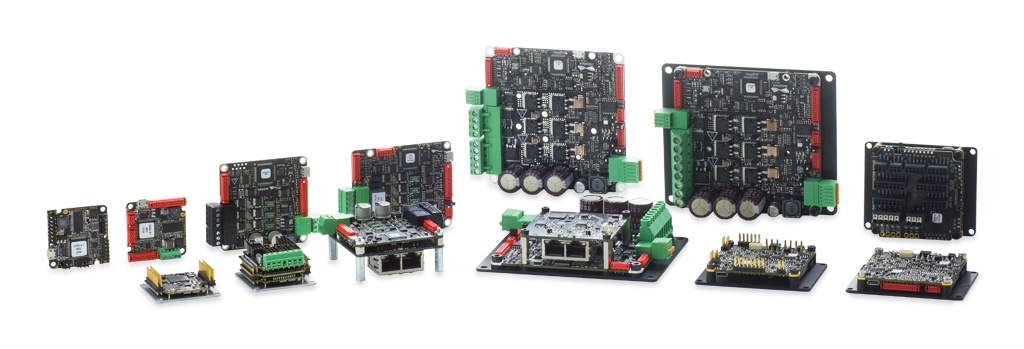
\includegraphics[width=\textwidth]{ingenia-servos.png}
  \end{figure}
\end{frame}

\begin{frame}
  \frametitle{What we wanted/needed}

  \begin{itemize}
    \item<1-> A \textbf{multiplatform library to communicate} with Ingenia's
      servo drives and perform some \textbf{motion control} tasks
    \item<2-> A library for our \textbf{configuration software}, but at the same
      time for \textbf{testing} or \textbf{automating} tasks
    \item<3-> A library that our \textbf{customers} can use for their typical
      applications
    \item<4-> A \textbf{single code base}, cannot maintain too many libraries
    \item<5-> An \textbf{easy to learn language}, with a \textbf{strong
      community} and lots of resources
  \end{itemize}
\end{frame}

\begin{frame}
  \frametitle{The reality}
  \begin{itemize}
    \item<1-> We love Python, but \textbf{not everybody in the world does}
    \item<2-> \textbf{Automation industry} is really \textbf{conservative},
      non-friendly to changes
    \item<3-> Most of our \textbf{customers are not up to date} with today's
      development practices
    \item<4-> Customers \textbf{still with PLC (sigh), VB, VB.NET, Win32-like
      APIs} and similar crap
  \end{itemize}
\end{frame}

\begin{frame}
  \frametitle{Our approach}

  \begin{itemize}
    \item<1-> Create a \textbf{library in C}, \textbf{object-oriented},
      targetting \textbf{Windows, Linux and macOS}
    \begin{itemize}
      \item<2-> Allows to \textbf{speed-up and fine-tune critical areas}
      \item<3-> Can create \textbf{wrappers to virtually any language} if
        needed, not tied to Python
      \item<4-> \textbf{Core code} (e.g. protocol, motion) in a \textbf{single
        code base}
    \end{itemize}
    \item<5-> Use \texttt{cffi} to create a \textit{native} Python extension
    \item<6-> Create a \textbf{class-based API in Python} on top of the native
      extension
  \end{itemize}

  \onslide<7->{\begin{center}
    \faGithub \\
    \href{https://github.com/ingenialink}{https://github.com/ingenialink} \\
    \href{https://github.com/ingenialink-python}{https://github.com/ingenialink-python}
  \end{center}}
\end{frame}

\begin{frame}
  \frametitle{How the extension is built}

  \begin{figure}
    \centering
    \tikzstyle{box}=[draw, minimum size=3em, rounded corners=0.3em, align=center]

    \begin{tikzpicture}[node distance=2cm,auto,>=latex']
      \node [box] (setup) {\texttt{setup.py} $\rightarrow$ \texttt{cffi\_modules}};
      \node [box] (build) [below of=setup] {Build script: \texttt{ingenialink\_build.py}};
      \node [box] (script) [below of=build]
        {\texttt{git clone} C library (and dependencies)\\
         Build libraries as \textbf{static, but PIC}\\
         Extract \textbf{declarations automatically from headers}\\
         Invoke \texttt{cffi}, linking with the built libraries};
      \node [box] (result) [below of=script]
        {Native extension with \texttt{ingenialink} \textbf{embedded}};

      \draw[->] (setup) -- (build);
      \draw[->] (build) -- (script);
      \draw[->] (script) -- (result);
    \end{tikzpicture}
  \end{figure}
\end{frame}

\begin{frame}
  \frametitle{Problems we have faced}

  \begin{itemize}
    \item<1-> Dealing with \textbf{multiplatform libraries is not that nice in
      C}
    \item<2-> Python GC (\textit{Garbage Collector}) may \textbf{not necessarily
      destroy objects in order when exiting} and we have object dependencies
      (e.g. \texttt{Servo} depends on \texttt{Network} resources)
    \item<3-> Linux binary wheels \textbf{need to be built using an ancient
      CentOS image}, which does not come with one of our dependencies (part of
      \texttt{systemd})
  \end{itemize}
\end{frame}

\begin{frame}[fragile]
  \frametitle{Example}

  \begin{minted}[fontsize=\scriptsize]{C}
    #include <ingenalink/ingenialink.h>

    double position;

    il_net_t *net = il_net_create("/dev/ttyACM0");
    il_servo_t *servo = il_servo_create(net, ID, TIMEOUT);

    il_servo_read(servo, &IL_REG_POS_ACT, &position);
    printf("Position: %.2f\n", position);

    il_servo_destroy(servo);
    il_net_destroy(net);
  \end{minted}

  becomes...

  \begin{minted}[fontsize=\scriptsize]{python}
    import ingenalink as il
    from ingenalink import regs

    net = il.Network('/dev/ttyACM0')
    servo = il.Servo(net, ID)

    position = servo.read(regs.POS_ACT)
    print('Position: {.2f}'.format(position))
  \end{minted}
\end{frame}

\begin{frame}
  \frametitle{Application Example}

  \begin{figure}
    \centering
    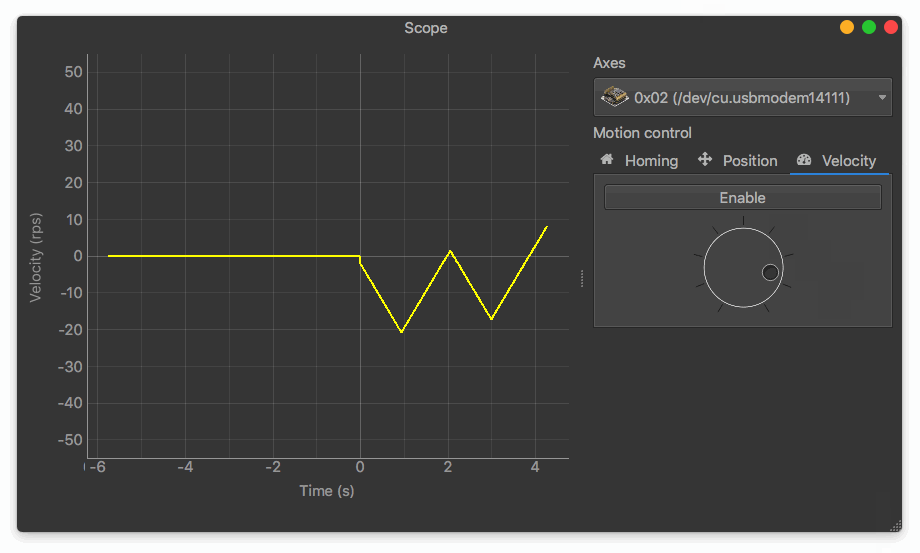
\includegraphics[scale=0.3]{example-scope.png}
    \caption{Application example (uses PyQt/PySide and pyqtgraph)}
  \end{figure}
\end{frame}

\section{Conclusions}

\begin{frame}[plain]{}
  \begin{center}
    \Huge \textbf{Conclusions}
  \end{center}
\end{frame}

\begin{frame}
  \frametitle{Conclusions}

  \begin{itemize}
    \item<1-> \texttt{cffi} allows to create \textbf{\textit{native-like}
      extensions with no effort}
    \item<2-> \textbf{Data types} and \textbf{function declarations} can be
      \textbf{\textit{copy-pasted} from headers} or even directly extracted
    \item<3-> \texttt{cffi} API level extensions require compilation, although
      binary \textbf{wheels} remove the requirement to the end-user
    \item<4-> \texttt{cffi} can be used in \textbf{ABI} mode (like
      \texttt{ctypes}) or \textbf{API} mode (like native extensions) seamlessly
    \item<5-> With \texttt{cffi} we can \textbf{directly define C functions} for
      critical parts with no need to create a shared library
    \item<6-> We can create a \textbf{single code base in C}, then wrap to
      \textit{any language}
  \end{itemize}
\end{frame}

\begin{frame}[c]
  \begin{center}
    \huge
    \textbf{THANK YOU!} \\
    Questions? \\
    \vspace{2cm}
    \normalsize
    \faGithub~\href{https://github.com/gmarull/pybcn-cffi}{https://github.com/gmarull/pybcn-cffi}
  \end{center}
\end{frame}

\end{document}
